\chapter{Wstęp}
\label{chapter:intro}

W~ramach pracy rozpatrywany jest problem weryfikacji postępów prac studentów dla projektu informatycznego, gdzie mamy zdefiniowane kilka grup projektowych.
Każdy z~zespołów, podczas trwania semestru, wykonuje taki sam rodzaj projektu.
Studenci przybliżają się do jego ukończenia poprzez zaliczanie kolejnych etapów.
Przykładem takiego przedmiotu są między innymi ”Podstawy Programowania”, prowadzone na wydziale Elektroniki i Technik Informacyjnych.

W pierwszym podrozdziale omówiono potrzebę oraz korzyści płynące z realizowania projektów grupowych w ramach programu studiów. 
Przedstawiony również został kierunek, w jakim będą zmierzać przedmioty projektowe w myśl reformy edukacji z roku 2018.

W podrozdziale \ref{programs-testing} omówiono sposoby oceny prawidłowości działania aplikacji.
Opisano tam również potrzebę nauki umiejętności testowania aplikacji przez studentów studiów informatycznych.

Kolejny podrozdział opisuje aktualny proces weryfikacji pracy studentów dla rozpatrywanych projektów grupowych.
Przybliżone są w nim problemy, na jakie napotykają prowadzący oraz studenci uczestniczący w tego typu przedmiocie.


Podrozdział \ref{tools} zawiera przegląd dostępnych, istniejących narzędzi wspomagających weryfikację umiejętności programistycznych użytkowników oraz ich zastosowanie w branży informatycznej.

W ostatniej sekcji zostało zamieszczone podsumowanie.

\vfill

\section{Projekty grupowe}

Prowadzenie projektów grupowych niesie ze sobą wiele korzyści.
Na podstawie obserwacji obecnego rynku IT (ang. Information Technology) można stwierdzić, że większość komercyjnych projektów to projekty zespołowe.
Uczestnicząc w~projekcie grupowym w~ramach zajęć, student przystosowuje się do warunków, z~jakimi zetknie się w~swojej pierwszej pracy.

Projekt zespołowy pozwala na naukę pracy w grupie.
Wymusza na studentach komunikację zarówno z członkami zespołu, jak i z prowadzącym.
Kształtuje umiejętność analizy, właściwego podziału zadań oraz estymacji czasu ich wykonania.
Studenci uczą się również odpowiedzialności nie tylko za swoją pracę, ale również za efekty całego zespołu.
Niejednokrotnie biorą też udział w rozwiązywaniu konfliktów w grupie.
Wszystkie powyżej wymienione kompetencje są istotne podczas pracy zawodowej.


Umiejętność pracy w grupie jest bardzo pożądana przez pracodawców.
W ramach pracy \cite{soft-skills} zgrupowano i poddano ocenie miękkie umiejętności, jakimi powinni posługiwać się pracownicy branży IT.
Badania zostały przeprowadzone na podstawie analizy wymagań zawartych w 650 ofertach pracy z uwzględnieniem różnych lokalizacji.
Wyróżniono cztery kategorie stanowisk: analityk systemowy, projektant oprogramowania, programista oraz tester.
Dla każdego ze stanowisk najczęściej wymaganą cechą jest komunikatywność.
Praca w grupie jest kolejną wskazywaną miękką umiejętnością.
Jest ona ceniona wyżej niż samodzielność w wykonywaniu zadań.
Zestawienie pożądanych umiejętności miękkich, jakimi powinni posługiwać się programiści, uzyskanych w ramach pracy F.~Ahmed zostało przedstawione na rysunku \ref{fig:soft-skills}.

\begin{figure}[h]
    \centering
    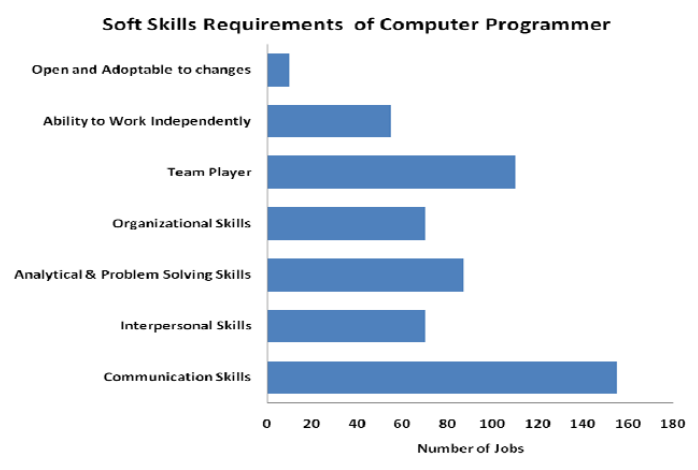
\includegraphics[width = 13cm]{chapter02/soft-skills.png}
    \caption{Pożądane umiejętności miękkie, jakimi powinni posługiwać się programiści (źródło \cite{soft-skills}).}
    \label{fig:soft-skills}
\end{figure}

Również wśród czterech wartości będących filarami metodyki Agile, zawartymi w manifeście, dwie z nich odnoszą się bezpośrednio do komunikacji.
W myśl założeń zwinnego podejścia do wytwarzania oprogramowania przedkłada się ludzi i interakcje ponad narzędzia i procesy oraz współpracę z klientem ponad negocjacje umów \cite{agile-manifesto}.
Umiejętność komunikacji można szlifować zarówno przez wspólną pracę w ramach zespołu, jak i dialog z prowadzącym.

Korzyści z projektów grupowych nie odnoszą się tylko do polepszenia umiejętności miękkich uczestników projektu.
Z założenia grupę projektową tworzą różne osoby, z których każda ma inne, własne zaplecze wiedzy technicznej.
Poprzez pracę w grupie studenci mają możliwość wymienienia się swoimi doświadczeniami i wiedzą.
Co więcej, mogą spojrzeć na ten sam, zadany problem z różnych perspektyw i dojść do odrębnych wniosków.
Może to znacznie skrócić czas wykonania zadania i wyeliminować błędy na wczesnym etapie. 
Wymiana doświadczeń i dyskusje na temat różnych podejść do zadanego problemu mogą również rzutować na lepsze podejście do rozwiązywania zadań w~przyszłości.

W myśl ustawy ”Prawo o szkolnictwie wyższym i nauce” z dnia 20 lipca 2018 \cite{higher-education-law}, od semestru zima 2019, w ramach programu studiów będzie kładziony nacisk na prowadzenie projektów grupowych.
Jest to podyktowane dążeniem do zapewnienia wysokiej jakości kształcenia oraz właściwego przygotowania do wykonywania zawodu.

\vfill

TODO: (FIX) Do tej pory było o tym, czemu warto opierać naukę na projektach zespołowych (i z tego wynika sens Pani pracy - czemu w ogóle zajmować się takim obszarem). Warto też wspomnieć krótko, że wiąże się z tm jednak wiele problemów, w szczególności dotyczących oceny, podtrzymywania motywacji, itp. - co zostanie omówione w dalszej części tego rozdziału.

\section{Sposoby oceny działania aplikacji}
\label{programs-testing}

Ważnym elementem oceny rezultatu pracy grupy studentów jest zweryfikowanie poprawności działania programów dla zadanych danych wejściowych.

Można byłoby oczekiwać, aby studenci sami dodawaliby przypadki testowe dla swoich aplikacji.
Podczas prezentacji programów prowadzącemu do ich zadania należałoby udowodnić, że kończą się one pozytywnym wynikiem.
Niestety ciężko ocenić trafność napisanych przez studentów przypadków testowych.
Podjęcie się takiego zadania przez prowadzącego wymagałoby od niego jeszcze bardziej indywidualnego podejścia do weryfikacji pracy grupy niż obecnie, w przypadku sprawdzenia wyniku działania samego programu.
Jest to związane między innymi z tym, że część napisanych przez studentów testów mogłaby się powtarzać.
Aby poprawnie ocenić jakość przypadków testowych należałoby rozważyć  między innymi priorytetyzajcę testowanych funkcjonalności, użyte narzędzia i poprawność asercji.
Samo zadanie napisania testów dla tworzonego programu mogłoby się okazać wyjątkowo ciężkie do zrealizowania w przypadku studentów, którzy są dopiero na początku swojej kariery programistycznej.
Takie osoby dopiero uczą się struktur języka i bardzo często nie mają wystarczająco dużo wiedzy, aby napisać poprawnie testy \cite{tests-and-begginers}.

Na podstawie wyników ankiety portalu Stack Overflow z roku 2019 widać, że umiejętność testowania kodu jest bardzo istotna w przyszłej pracy \cite{stack-overflow-survey}.
W ramach badania zapytano ankietowanych, czy w ich miejscach pracy używa się testów jednostkowych podczas wytwarzania oprogramowania.
Na rysunku \ref{fig:unit-tests-use} przedstawiono wyniki ankiety.
W~przybliżeniu jeden na trzech ankietowanych nie używa testów najniższego poziomu w swoim procesie, ale zaledwie 4.4\% jest zadowolna z takiego podejścia.
95.6\% osób testuje jednostkowo swoje aplikacje lub uważa, że ten rodzaj testów byłby przydatny w procesie wytwarzania oprogramowania.
Warty uwagi jest również rezultat otrzymany w powiązaniu używania testów jednostkowych z poziomem satysfakcji z pracy ankietowanych, który został przedstawiony na rysunku \ref{fig:unit-tests-satisfaction}.
Osoby używające tego rodzaju testów są bardziej zadowolone ze swojej pracy.

\begin{figure}[h]
    \centering
    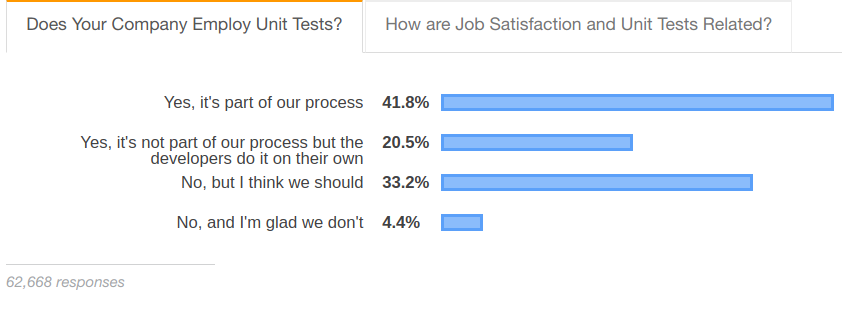
\includegraphics[width = 13cm]{chapter02/unit-tests-use.png}
    \caption{Używanie testów jednostkowych w procesie wytwarzania oprogramowania (źródło: \cite{stack-overflow-survey}).}
    \label{fig:unit-tests-use}
\end{figure}

\begin{figure}[h]
    \centering
    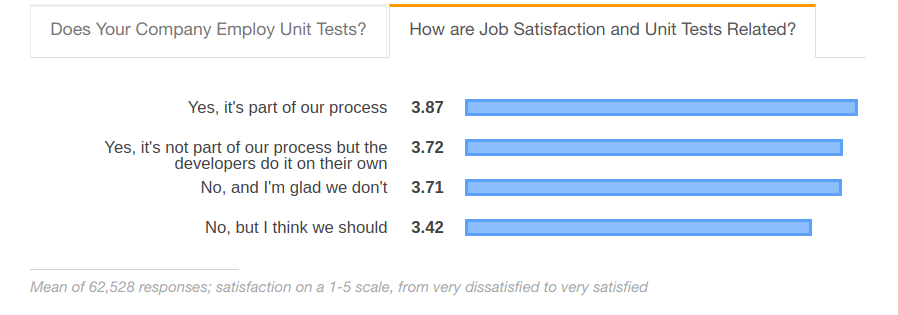
\includegraphics[width = 13cm]{chapter02/unit-tests-satisfaction.png}
    \caption{Powiązanie używania testów jednostkowych i zadowolenia z pracy (źródło: \cite{stack-overflow-survey}).}
    \label{fig:unit-tests-satisfaction}
\end{figure}

Umiejętność testowania kodu jest często sprawdzana podczas procesu rekrutacyjnego.
Zarówno w przypadku, gdy kandydat ma za zadanie zaimplementować małe zdanie algorytmiczne, jak i napisać działającą aplikację.
W obu przypadkach musi on udowodnić poprawność swojego rozwiązania poprzez testy.
Niezależnie czy poprzez analizę słowną przebiegu działania programu, czy przez zaimplementowane testy wewnątrz aplikacji.
W~pozycji pomagającej przygotować się do procesu rekrutacji ”Cracking the coding interview” \cite{cracking-the-coding-interview} testowaniu został poświęcony odrębny rozdział.

Programiści ćwiczący umiejętność testowania aplikacji potrafią lepiej wychwytywać potencjalne błędy na wczesnym etapie tworzenia oprogramowania \cite{testing-better-error-catch}.
W przypadku małych i średnich firm wytwarzających oprogramowanie z wykorzystaniem podejścia Agile, często nie ma oddzielnych zespołów testerów.
W takich software house'ach zadaniem inżyniera oprogramowanie jest nie tylko napisanie działającej funkcjonalność, ale również samodzielne przetestowanie jej, poprzez testy jednostkowe i integracyjne.
W dużych korporacjach wykorzystujących metodyki Agile umiejętność testowania jest również istotna ze względu na ścisłą współpracę między interdyscyplinarnymi członkami zespołu.

Wśród wartości fundamentalnych dla podejścia XP (ang. Extreme Programming) do wytwarzania oprogramowania jest wymieniona informacja zwrotna (ang. feedback) \cite{extreem-programming}.
Opisywana jest ona jako szybkość oceny poprawności dodawanego kodu i jego interakcji z innymi częściami systemu oraz oszacowania regresji.
Szybką informację zwrotną dotyczącą dodawanej funkcjonalności można osiągnąć między innymi przez utrzymywanie poprawnych przypadków testowych.

W literaturze można znaleźć wiele prac poświęconych testowaniu programów i wprowadzaniu nauki umiejętności testowania w ramach programu studiów.
Kładziony jest coraz większy nacisk na tę umiejętność \cite{tests-important}.
Wśród zamieszczonych opinii powszechną jest, że testowanie aplikacji jest ważne i potrzebne od samego początku studiów \cite{test-from-scratch}.
Wśród propozycji można znaleźć pomysł nauki pisania programów w metodyce TDD (ang. Test Driven Development) już od pierwszego semestru studiów \cite{tdd-on-start}.
Wymagałoby to jednak wysokich kwalifikacji prowadzących co do znajomości metodyki i jej praktyki.
Warto zaznaczyć, że TDD opiera się na pisaniu testów jednostkowych, co, jak zostało wspomniane wcześniej, wymaga wiedzy na temat programowania.

Jak zostało napisane wcześniej, studentom rozpoczynającym naukę programowania bardzo ciężko byłoby napisać odpowiednie testy do swoich programów.
Praktycznie niemożliwe jest też wprowadzenie na początku studiów całego przedmiotu poświęconego nauce pisania testów, ze względu na przepełniony obecnie program studiów \cite{overflow-studies-program}.
Warto jednak pokazywać studentom zalety testowania aplikacji.
Można to osiągnąć między innymi przez dostarczanie studentom zdefiniowanych przez prowadzących poprawnych przypadków testowych dla ich programów.

W zależności od poziomu złożoności aplikacji wysokie pokrycie testowe mogłoby być jednak trudne do utrzymania.
Wraz ze wzrostem skomplikowania programów tworzenie przypadków testowych przez prowadzących stawałoby się coraz bardziej czasochłonne.

Ciekawym pomysłem zmniejszenia czasu potrzebnego na dodawanie testów jest zobligowanie studentów do samodzielnego pisania przypadków testowych, zebranie wszystkich testów i uruchomienie programu każdej grupy dla wszystkich zebranych przypadków.
Słuszność takiego podejścia została opisana w artykule \cite{write-tests-by-students}.
Warto jednak zaznaczyć, że zadaniem prowadzącego w tym przypadku byłaby ocena jakości przypadków testowych.
Dodatkowo mogłoby się okazać, że zbiór testów ma stosunkowo niskie pokrycie, co jest wysoce prawdopodobne w przypadku studentów rozpoczynających naukę programowania.
Można jednak oczekiwać, że im większe doświadczenie studentów tym lepsze pokrycie testami aplikacji osiągniemy.

Innym pomysłem na zmniejszenie czasochłonności tworzenia testów akceptacyjnych jest porównywanie wyników programów studentów ze wzorcowym programem prowadzącego uruchomionym dla tych samych danych wejściowych.
W tym przypadku dane wejściowe mogłyby być generowane losowo.
Ten sposób chroniłby przed próbą sztywnej implementacji programu, która generowałaby właściwy wynik tylko dla znanych wcześniej przypadków testowych.
To podejście ma też swoje wady, ponieważ używając zwykłego generatora losowego można uzyskać bardzo niskie pokrycie i nie przetestować poprawnie przypadków brzegowych.

Kolejnym innowacyjnym podejściem jest wykorzystanie metod ML (ang. Machine Learning) do generowania przypadków testowych.
Ta metoda została opisana w pracy doktorskiej \cite{teach-testing-thesis}.
Dzięki uczeniu maszynowemu z wykorzystaniem prac studentów z poprzednich lat uzyskano narzędzie pozwalające generować przypadki testowe z bardzo wysokim pokryciem.
Trudno byłoby jednak zastosować podobną metodę w ramach proponowanej platformy, ze względu na brak dostępnych i dobrze opisanych programów studentów poprzednich lat.



\section{Proces weryfikacji pracy studentów}

Obecnie proces weryfikacji pracy studentów nad projektem zespołowym podczas semestru jest czasochłonny.
Każdy z prowadzących ma pod swoją opieką kilka (w przypadku przedmiotu "Podstawy Programowania" najczęściej od pięciu do siedmiu) grup projektowych.
W skład każdej grupy wchodzi kilku studentów.
Projekt jest podzielony na etapy. 
W przypadku przedmiotu podstawy programowania odbyło się sześć faz, każda zakończona przesłaniem sprawozdania.

Poszczególne zadania wykonywane przez studentów są oceniane indywidualnie, pomimo powtarzalności problemów, jakie mają do rozwiązania zespoły.
W celu oceny pracy w ramach jednego etapu prowadzący przegląda kod zamieszczony przez studentów w systemie kontroli wersji, ocenia sprawozdanie oraz przeprowadza spotkanie ze studentami.
Przy ocenie postępów prowadzący bazuje na prezentacji programu wykonanej przez studentów lub na własnych doświadczeniach z interakcji z programem.

Przedstawienie prowadzącemu wyników cząstkowych oraz końcowych przez studentów może okazać się kłopotliwe.
Manualne uruchamianie programów na prywatnych maszynach studentów jest czasochłonne.
Dodatkowo podczas przedstawiania wyników, mogą zaistnieć komplikacje związane między innymi z niepoprawną konfiguracją środowiska uruchomieniowego lub niewłaściwym doborem przypadków testowych.
W sytuacji, gdy zadaniem studentów jest zaprezentowanie interakcji pomiędzy stworzonymi przez nich modułami programów, prawdopodobieństwo wystąpienia powyższych błędów wzrasta.
Prowadzący, decydując się na samodzielne uruchomienie programów studentów, w~celu ich oceny, jest również narażony na powyższe sytuacje.
W przypadku niedokładnej dokumentacji dotyczącej pracy studentów, jego zadanie może zostać znacznie utrudnione.
Taka sytuacja może doprowadzić do uzyskania niskiego wyniku przez studentów mimo niewielkich błędów w implementacji lub błędnie zrozumianych założeń.
Ze względu na indywidualne podejście do każdego z zespołów i etapów proces weryfikacji jest czasochłonny.

Studenci otrzymują informację dotyczącą oceny danego etapu, po jego zakończeniu.
W trakcie zadania oczywiście mogą doprecyzować szczegóły z prowadzącym.
Zdarza się jednak, że pomimo dodatkowego uszczegółowienia, niektóre założenia są przez studentów zrozumiane w inny sposób niż oczekiwałby tego prowadzący.
W takim przypadku studenci podczas trwania etapu mogą napisać program zgodny z błędnie rozumianymi założeniami i dopiero po złożeniu kompletnego sprawozdania z etapu dowiedzieć się o niepoprawnej interpretacji zadania.
Dla obecnego procesu prowadzenia projektu informacja zwrotna dotycząca postępów pracy dociera do studentów stosunkowo późno.

Podczas prowadzenia projektu prowadzący napotykają również na problem braku systematycznej pracy studentów podczas semestru.
Może on wynikać częściowo z nie posiadania oficjalnej wiedzy o aktualnych postępach innych grup.
Podgląd statusu prac pozostałych zespołów mógłby być dodatkową motywacją dla studentów do podjęcia działań i wykonania danego etapu.

Proces prowadzenia projektów grupowych jest aktualnie modernizowany.
Dla przedmiotu ”Podstawy Programowania” wśród wprowadzanych usprawnień można wyróżnić między innymi zobligowanie studentów do zamieszczania kodu swoich aplikacji w systemie kontroli wersji GitLab.
Jest to istotna modernizacja pozwalająca na lepsze zarządzanie kodem programów i jego archiwizację.
Jednak studenci (zwłaszcza pierwszych lat studiów) nie potrafią w pełni wykorzystać zalet tego narzędzia i poprawnie z niego korzystać.
Często nie zamieszczają kodu w postaci małych czytelnych commit'ów.
Zamiast tego zamieszczają całe archiwa z nowymi wersjami oprogramowania.
Dokumentacja programów również nie jest zawsze pełna.
Usprawnienie w postaci systemu kontroli wersji ułatwia dostęp do kodu programów studentów i pozwala przeglądać go na przystosowanym do tego interfejsie.
Nie eliminuje to jednak czasochłonnego, indywidualnego podejścia do oceny każdej z grup i etapu.

Dzięki wprowadzeniu systemu kontroli wersji można uzyskać szereg statystyk dotyczących pracy studentów.
Nie są to jednak pełne informacje, które mogłyby interesować prowadzącego.
Sam kod zamieszczany w systemie, nie jest wystarczający do oceny etapu.
Co więcej, jego samodzielna analiza nie poprawiłaby, a być może nawet pogorszyła, czasochłonność weryfikacji wyników cząstkowych.
Ważnym elementem oceny poszczególnych etapów jest ocena poprawności działania uruchomionych programów dla zadanych danych wejściowych.


\section{Narzędzia wspomagające ocenę umiejętności programistycznych}
\label{tools}

Obecnie istnieje wiele narzędzi wspomagających ocenę umiejętności programistycznych użytkowników.
Są to najczęściej platformy z interfejsem webowych dostępne dla wszystkich.
Ogólna zasada działania tych narzędzi sprowadza się do napisania przez użytkownika prostego, odseparowanego programu z zadaną wejściową sygnaturą.
Następnie kod jest kompilowany, budowany i przepuszczany przez szereg testów akceptacyjnych.
Wynik testów jest przedstawiany użytkownikowi w postaci prostej wizualizacji.

Wśród narzędzi można wyróżnić strony umożliwiające testowanie umiejętności algorytmicznych użytkowników.
Pozwalają one zarówno na sprawdzenie poprawności wykonania implementowanych algorytmów, jak i oceny ich złożoności.
Wśród takich platform można wyróżnić między innymi: Codility \cite{codility} i HackerRank \cite{hacker-rank}. 
Pozwalają one także na przeprowadzanie zawodów w szybkim tworzeniu poprawnych i efektywnych algorytmów. 
Słuszność takich platform można potwierdzić między innymi na podstawie tego, że duże międzynarodowe korporacje takie jak Google zachęcają do przygotowywania się do procesów rekrutacyjnych z użyciem stron tego rodzaju. 
Niektóre mniejsze firmy prowadzą początkowe etapy rekrutacji z wykorzystaniem tych platform.

Innym rodzajem narzędzi są strony umożliwiające naukę programowania lub naukę programowania we wskazanym języku. 
Mogą być to proste symulatory środowisk, gdzie wraz z kolejnym etapem kursu użytkownik ma za zadanie napisać niewielki program lub jego część.
Czasem jednak narzędzia są bardziej rozbudowane i pozwalają na wizualizację działania programów w formie gry np. GameCoder \cite{game-coder}.
Podejście z tworzeniem gier jest wykorzystywane w celu zachęcenia i zainteresowania użytkowników oraz lepszego zobrazowania wyniku działania ich kodu.
Wśród narzędzi mających na celu lepsze zrozumienie wykonania kodu przez wizualizację można wyróżnić platformę do nauki programowania równoległego opisaną w artykule \cite{pharaller-platform}.

W ramach pracy doktorskiej \cite{teach-testing-thesis} opisano narzędzie pozwalające na naukę pisania testów jednostkowych.
Bazując na danych historycznych, zaproponowano platformę pozwalającą na ocenę jakości testów pisanych przez użytkowników.
Jest to bardzo ciekawe i godne uwagi podejście do oceny umiejętności testowania programów przez studentów.

Narzędzia wspomagające ocenę umiejętności programistycznych są powszechne i~mają różne zastosowania.
Skupiają się one jednak na niewielkich, pojedynczych, indywidualnych zadaniach.
Ze względu na powyższe cechy użycie ich w ramach wieloetapowego, długoterminowego i grupowego projektu nie pomoże znacząco usprawnić procesu weryfikacji pracy studentów.
W ramach pracy zaimplementowano i zbadano platformę umożliwiającą lepszą ocenę całego procesu tworzenia projektu z uwzględnieniem każdego etapu.
Proponowane rozwiązanie jest generyczne i poprzez odpowiednie zdefiniowanie środowiska uruchomieniowego może zostać użyte dla dowolnego języka programowania na każdym etapie studiów.

\vfill


\section{Podsumowanie}

TODO: Napisać podsumowanie